\documentclass[letterpaper,12pt]{article}
\usepackage{utr}
\usepackage{graphicx}
\usepackage{url}
%
\title{Replacing Unicon's Random\\ Number Generator}
\author{Don Ward}
\trnumber{??}
\date{2019-08-20}
%
\begin{document}
\abstract{
% The normal typeface means that the front matter overflows into two pages.
% Presumably, the abstract is too prolix for its own good, but it is
% difficult to condense it further.
%
% Even with \small, the front matter is two pages (but the second page is
% blank, which is slightly better).
%
% But, with a blank affiliation, all is well.
\affiliation{~}
{\small
This report discusses whether the random number generator used by Unicon
should be replaced and, if so, with what. The report concludes that the
best option would be to provide an extensible portfolio of generators with
different characteristics and leave the choice of which one to employ to
the user. It also suggests a possible implementation.
}
}
\maketitle
%
% The &random keyword is used a lot, so save some typing
\newcommand{\rndkwd}{{\sf \&random}\ }
% If the name "rnglib" is changed, don't forget to also replace it
% in the verbatim environments
\newcommand{\rndlibkwd}{{\sf \&rnglib}\ }
% A convenient way to get a consistent style of error messages.
\newcommand{\UniconError}[2]{{\sf#1} --- {\sf #2}}
% Smaller urls
\newcommand{\surl}[1]{{\small\url{#1}}}
%
\section{Introduction}
The ``{\sf Help Wanted!}'' page of \surl{www.unicon.org}
contains the following item:
\begin{quote}
  {\sf
  {\bf Improve random number generator (S) }
  --- Unicon should consider changing its random number generator to use a
  Mersenne twister. What are the pros and cons?  A first step would be to
  acquire or develop an implementation that is suitable.
  }
\end{quote}
This is the second draft of a report that summarizes the advantages and
disadvantages of a replacement random number generator (RNG).
In some respects, it exceeds its brief by discussing other generators
alongside the Mersenne Twister.

All but one of the generators discussed later are {\em pseudo} random rather
than genuinely random%
\footnote{
  A genuinely random generator requires access to a high quality supply of
  entropy provided either by hardware, often external, or by using software
  that gathers entropy from the operation of the computer system itself
  such as the \texttt{/dev/random} device in modern Unix systems.
}.
For this reason, the abbreviation PRNG will usually be used in the rest of
this report.

There is no consensus on how to rate the quality of a PRNG: that is, given
a collection of PRNGs, there is no generally accepted method to rank them in
strict order from ``lowest quality'' to ``highest quality''.
%
Several aspects of quality (such as randomness, resistance to
cryptanalysis, speed etc.)  are in play and people disagree about which is
most important --- in some cases the relative importance of the factors to
consider depends on the application --- so the best that can be achieved is
a partial ordering. Everyone might be able to agree that a particular
subset of PRNGs are all better than another subset, whilst disagreeing
about the relative ordering within the subsets themselves.

This, perhaps regrettable, lack of consensus motivates the proposals made
later on in this document, which would allow the choice of PRNG to be made
by the user%
\footnote{
  ``User'' here means ``system designer'' or ``programmer'' although, if
  the design of the application program permits it (and it is possible to
  choose at run time), it could also mean the actual user of the Unicon
  application.
}.

Before considering the Mersenne Twister PRNG and others, it is useful to
list the advantages and disadvantages of {\em any} replacement PRNG.

\section{The Pros and Cons of changing the PRNG}

There are some aspects of a replacement that are common to all
candidates. That is, they are more to do with the change itself than the
characteristics of a particular algorithm. This section discusses those
aspects.

\newcommand{\GoodThing}{\protect{\makebox[20pt][l]{$\oplus$}}}
\newcommand{\BadThing}{\protect{\makebox[20pt][l]{$\ominus$}}}
\newcommand{\PossiblyGoodThing}{\protect{\makebox[20pt][l]{$\oplus$?}}}
\newcommand{\PossiblyBadThing}{\protect{\makebox[20pt][l]{$\ominus$?}}}

Each of the following topics will be labelled with a ``$\oplus$'' denoting
something that is considered advantageous or a ``$\ominus$'' denoting a
disadvantage.  Sometimes, if the issue is not so clear-cut or if there are
differing opinions about its relevance, a ``{\bf ?}''  will be appended to
the label.

\begin{description}

\item[\GoodThing]
  Presumably, any new PRNG will be better than the existing
  algorithm --- nobody would want the replacement if it was
  worse. Possibilities for improvement include
  \begin{itemize}
  \item Longer period.
  \item Better results on statistical tests for randomness (i.e. pass more
    tests or pass more stringent tests).
  \item Better resistance to cryptanalysis.
  \item Faster or smaller (although this is unlikely, given the speed and
    extremely small state of the current algorithm).
  \item Compatibility with the PRNG used in other software.
  \end{itemize}

\item[\BadThing]
  Backwards incompatibility: many programs assign a seed to \rndkwd to get
  reproducible behaviour between runs.  Any replacement of the existing
  PRNG, which is used both by Unicon and by Icon, will mean that the output
  will not be same: Unicon programs using \rndkwd that are written in the
  Icon subset will produce different results on Icon and Unicon.

  This doesn't mean that the behaviour won't be reproducible --- the output
  will be the same between runs --- but it will be {\em different}
  reproducible behaviour on each platform. However, programs that depend on
  reproducible behaviour between this and previous versions of Unicon will
  definitely break%
  \footnote{
    This is not just a theoretical possibility: the author uses a DiceWare
    program, written in Unicon, that generates random passphrases based on
    the input credentials. The passphrases aren't written down anywhere,
    they are generated (again) when needed. Changing the PRNG would require
    that {\em every} passphrase be changed.
  }.

\item[\PossiblyBadThing]
  It is very likely that a replacement PRNG will be slower than the current
  one or will require more space for its state (or both). Resistance to
  cryptanalyis or better statistical properties practically {\em demand} more
  than 32 bits of state.

  Whether the increase in memory footprint or the decrease in speed has a
  perceptible impact on program performance is susceptible to
  experiment (and Appendix C makes a proposal to find out).
  If the experiments are done, they will need to be performed on as
  wide a range of target hardware as possible. The underlying hardware can
  have a surprisingly large impact on the {\em relative} as well as the
  absolute performance of PRNGs\cite{Bernstein:cypherSpeed}.

\end{description}

\subsection{Discussion: should the present PRNG be replaced?}

The designers of Unicon have usually been very careful to ensure that a
Unicon program that also happens to be an Icon program produces the same
results on both platforms%
\footnote{
  It is notable that the Unicon designers chose to depart from backwards
  compatibility in the very topic we are discussing --- the generation of
  random numbers. An Icon program that does not set the value of \rndkwd
  will always produce the same random sequence
  --- see \cite{IconBook} \S 5 page 66 ---
  the same code fed into a Unicon system will produce a different random
  sequence each time it is run. The reasons cited in the Unicon Book
  (chapter 4) come down to Unicon's behavour being more generally useful,
  and it's easy to restore the previous behaviour with one assignment.
}.

There needs to be a very good reason to break that backwards compatibility
and, for many people, a better PRNG will not necessarily be a good enough
reason, especially as the current PRNG is still satisfactory for many
purposes. Accordingly, the answer to a strict interpretation of the
question posed above is ``No'' --- Job done; now we can all go home and
relax; no further action is required.

However, a key insight is that replacement is not the only option. We could
make more than one PRNG available and somehow switch between them. The
choice could be implemented at run time or, possibly, at compile time.

In any event, if we do have a choice between PRNGs it is clear from the
strong desire to retain backwards compatibility that the current algorithm
should be one of the choices and, furthermore, it should be the default
choice. Explicit action should be required to switch to a new PRNG.

\subsection{Mission Creep}
If we have a choice between continuing to use the existing PRNG or
switching to the new one, the question ``why are there only two options?''
naturally arises. As mentioned in the introduction, there are different
opinions about which aspects of a PRNG are most important and it will be
very difficult to land on a single alternative that pleases most of the
people most of the time. But a small, judiciously chosen, collection
of PRNGs with differing characteristics might just do the job.

We can go further: if the mechanism to add PRNGs is {\em extensible}, so a
user may add to the available alternatives, the pressure to make the right
choice of PRNGs up-front is greatly reduced. As the state of the art
develops we can add new shinier PRNGs to the standard collection and users
with special requirements, or a pressing need for a newer algorithm, can
add their own at any time.

\section{Candidate PRNGs}
Where to start? A lot has happened in the field of random number generation
since the original Icon PRNG was chosen in the mid to late seventies.
Significant progress%
\footnote{
  An idea of how much progress can be got by comparing the second edition
  of Numerical Recipes \cite{PressEtAl:numericalRecipes-2} \S 7 (published
  in 1992) with the same chapter of the third edition
  \cite{PressEtAl:numericalRecipes} published in 2007.

  The references in this report are in approximate chronological order from
  oldest to newest. So a rough and ready guide to whether one reference is
  newer than another is to compare the reference numbers.
}
has been made since then and there are now many hundreds of generators from
which to make a selection. The problem is to winnow the hundreds of
candidates down to a manageable number. We should certainly include the
Mersenne Twister in the list for consideration, since that was the original
suggestion. A generator that is cryptographically secure might also be a
useful addition for some applications. 

\noindent
\begin{tabular*}{7in}{cc}
\begin{minipage}{3.4in}
A good starting point is to see what choices have been made by other
people, especially experts, although it might be wise to prefer recent
choices, over those made some time ago, because of the advances in the
field.  Another idea is to consult authoritative tomes such as
\cite{PressEtAl:numericalRecipes,Knuth:SemiNumerical3}.
The eSTREAM project%
\footnote{
The eSTREAM project\cite{eStream} was a multi-year effort, running from
2004 to 2008, to promote the design of efficient and compact stream ciphers
suitable for widespread adoption.
}
is a good source for candidate algorithms that are thought to be
cryptographically secure. The recommendations made by the GNU Scientific
Library \cite{GnuScientificLibrary} and the selection in the latest draft
of the C++ standard\cite{CplusplusStd:N4820} might also prove instructive.

\end{minipage}
&
\parbox{2.5in}{
  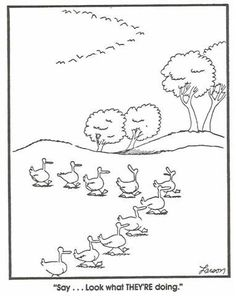
\includegraphics[width=2.5in,height=2.5in]{larson.jpg}
}
\end{tabular*}

It would be nice to follow the recommendations of NIST but experience ---
see \cite{Schneier:BackDoor} amongst many others --- suggests that it isn't
always a good choice.

\vspace{0.1in}

As a last resort we could roll our own generator, although history
indicates that would be a very bad idea indeed.  A quote from
\cite{PressEtAl:numericalRecipes-2} \S 7, which contains a devastating list
of examples of lousy PRNGs, seems apposite
\begin{quote}
  The historical record (of random number generators) is nothing if not
  appalling.
\end{quote}
It would be a brave decision to fly in the face of so much negative
evidence. In the early nineties --- at the time of writing of
\cite{PressEtAl:numericalRecipes-2} --- it might, just possibly, have been
a sensible thing to do. Not now.

A significant benefit of choosing somebody else's generator is that
somebody else has already done the work of evaluating the statistical
properties%
\footnote{
  If the technical paper (or other material) describing the generator
  doesn't mention statistical tests for randomness, such as
  Diehard\cite{Marsarglia:Diehard}
  or Dieharder\cite{Brown:Dieharder}
  or NIST--STS (a.k.a. NIST--SP 800-22)\cite{BassinghamEtAl:Statistical}
  or TESTU01\cite{McCullough:TESTU01,L'Ecuyer:TESTU01},
  then walk away.
}.
Everyone agrees that a new generator should undergo substantial testing
before being put to serious use. Some of the tests referred to in the
footnote will take {\em days} to complete a single test run.

Note that in the following sections describing each generator, all
generators are permissively licensed unless the description says otherwise.

%----------------------------------------
\subsection{Mersenne Twister (MT)}
The Mersenne Twister was invented in 1997 and was designed to avoid the
deficiencies of most of the PRNGs extant at the time. It is described in
\cite{Matsumoto:MersenneTwister}.
\begin{description}
\item[\GoodThing]
  Extremely long period ($2^{19937} - 1 \simeq 4.3 \times 10^{6001}$).
\item[\GoodThing]
  Quite fast; perhaps not as fast as some others, but certainly in the same ballpark.
\item[\GoodThing]
  In very wide use. Chosen for inclusion into the GNU Scientific Library,
  the C++ standard library and many others.
\item[\GoodThing]
  Very good statistical properties.
\item[\PossiblyBadThing]
  Not cryptographically secure --- there is a secure variant, called
  CryptMT, but it is patented. CryptMT is free for non commercial use,
  but incorporating it into Unicon might restrict the availability of
  Unicon to commercial users --- note this does not apply to MT itself: that
  is free to use for everyone.
\item[\PossiblyBadThing]
  The original algorithm was slow to recover from a bad seed (one with a
  high proportion of zero bits). ``Slow'' in this context means up to $7
  \times 10^5$ iterations. A 2002 update to the algorithm now makes the
  possibility of starting in a bad state ``very unlikely'' --- although it
  does not preclude stumbling into it by accident.
  % ToDo: Add reference and find out if the mod always gets the same good
  % seed if fed the same bad seed.
\item[\PossiblyBadThing]
  It has a large state (2.5KB) compared to other generators, which is
  perhaps not so good for multi-threaded applications.

\item[\GoodThing]
  The random sequence can be efficiently advanced, by jumping ahead. This is
  particularly important when doing Monte Carlo simulations in parallel%
  \footnote{
    The basic problem is that parallel simulations should not share the
    same sequence of pseudorandom numbers, because that would destroy the
    assumption that the values produced in parallel are independant of each
    other. One idea is to use different seed values in each thread, but
    there is usually no guarantee that they might not collide --- perhaps
    after a short time --- and begin to use the same sequence, thus
    destroying the independence. A common way around this problem is to
    partition the random sequence into several disjoint sequences that are
    a {\em very} long way apart. \cite{HiroshiEtAl:EfficientJumping} gives
    details of an efficient way of doing this for MT and other similar
    algorithms.
  }.

\item[\PossiblyBadThing]
  CryptMT was one of the finalists in the eSTREAM project\cite{eStream} but
  didn't make the final cut.  The comments (in 2008) were:
  \begin{quote}
    {\sf
	CryptMT v3. The cipher CryptMT has a very unusual design which delivers
    very reasonable performance. While there have been no negative
    cryptanalytic results against the cipher in the last phase of eSTREAM,
    we are somewhat concerned that the security of the cipher, in
    particular the non-linear filter component, might not yet be as
    well-understood as some of the other finalists. We anticipate that
    elements of CryptMT will continue to be of interest to the
    cryptographic community, and we hope that the full advantages of the
    approach embodied in CryptMT v3 can be evaluated.  However, we are
    currently not sufficiently confident in the design and security of this
    algorithm for us to include it in the final portfolio.
    }
  \end{quote}
  Note that these comments are about CryptMT, not about MT itself.
  It doesn't make MT a bad PRNG, but the very existence of CryptMT implies
  that MT isn't suitable as the basis of a cryptographically secure stream
  cipher without the ``special sauce'' of a non-linear filter (and the
  eSTREAM comments raise some doubts%
  \footnote{
    Not too much should be made of this: cryptographers are a cautious
    bunch at the best of times.
    }
  even when such a filter is in use).

  An attempt to build a stream cipher based on the MT may run afoul of the
  cryptMT patents. However, there is a large amount of ``anecdata'' about
  good engineers (but not cryptographers) making a mess of things when they
  roll their own encryption, so perhaps an obstacle to doing so wouldn't be
  such a bad thing.
 
\end{description}
    
%----------------------------------------
\subsection{Rabbit (Rbt)}
Rabbit is from profile 1 (software)%
\footnote{
  The eSTREAM portfolio ciphers fall into two profiles. Profile 1
  contains stream ciphers more suitable for software applications with high
  throughput requirements. Profile 2 stream ciphers are particularly
  suitable for hardware applications with restricted resources such as
  limited storage, gate count, or power consumption.
}
of the eSTREAM project\cite{eStream}. It uses a 128 bit key and 64 bit IV to
initialize the generator which produces a stream of 128 bit blocks. Up to
$2^{64}$ blocks may be produced before a new key/IV pair is required%
\footnote{
  The reader may be wondering why a re-key is needed after this
  comparatively short number of operations compared to the period. The
  answer is to maintain the {\em security} of the cipher. When used as a
  normal (non-cryptographically secure) PRNG, the re-key is not required.
}.

\begin{description}
\item[\PossiblyGoodThing]
  Comparatively short period (compared to MT) of
  $2^{256}-1 \simeq 1.2 \times 10^{77}$,
  but still more than long enough for all practical purposes.
\item[\GoodThing]
  Fast (faster than MT on most processors, but not always
  faster\cite{Bernstein:cypherSpeed})
\item[\GoodThing]
  Fairly small state (513 bits, 65 bytes).
\item[\GoodThing]
  Chosen by eSTREAM --- i.e. selected by a consensus of people with
  expertise in the field.
\item[\PossiblyGoodThing]
  Cryptographically secure%
  \footnote{
    The {\bf ?} after the $\oplus$ doesn't mean there are doubts about its
    security, it means that some authorities consider that cryptographic
    security is not a requirement for a general purpose RNG.
    }
  (almost by definition).
\item[\GoodThing]
  Passes the statistical tests for randomness --- {\em all}
  cryptographically secure PRNGs pass the randomness tests.
\item[\GoodThing]
  Unchanged since 2003 which, given the scrutiny of the algorithm during
  the duration of the eSTREAM project and afterwards, lends
  credence to the claims of cryptographic security.
\item[\PossiblyBadThing]
  No method to advance the random sequence by jumping ahead. Not so good
  for Monte Carlo simulations in parallel.

\end{description}

%----------------------------------------
\subsection{Numerical Recipes \texttt{Ran}}
\texttt{Ran} is published in the third edition of Numerical Recipes
\cite{PressEtAl:numericalRecipes} \S 7. According to the authors it is
``our suspenders-and-belt, full-body-armour, never-any-doubt generator''
and will ``generate all the uniform deviates you will ever need''.
\begin{description}
\item[\GoodThing]
  Decently long period ($3.138 \times 10^{57}$).
\item[\PossiblyGoodThing]
  Fast%
  \footnote{
    The reason for the {\bf ?} is that it appears to be similar to the
    Wichmann--Hill generator (discussed next) which is reported to to be
    about five times slower than MT.
    }.
\item[\GoodThing]
  Small state (24 bytes).
\item[\GoodThing]
  Passes the standard statistical tests for randomness.
\item[\PossiblyGoodThing]
  Not ``overengineered''%
  \footnote{
    Numerical Recipes (2007), in a section discussing overengineering, contains
    the following advice ``Avoid using generators with period $>
    10^{100}$. You {\em really} will never need it and, above some minimum
    bound, the period of a generator has little to do with its quality''.
    Clearly, given the widespread use of MT, some people disagree. See also
    \cite{James:HighQualityRNGs}(2019) which says (amongst other requirements
    for the highest quality), ``Period must be long enough, $> 10^{100}$ ''.
  }.

\item[\PossiblyBadThing]
  Not cryptographically secure%
  \footnote{
    The section referred to in the previous footnote also advises against
    generators that are ``(over)designed for cryptographic use'', but we
    should remember that the focus of the book is numerical algorithms for
    scientific computing and, from that limited perspective, a
    cryptographically secure PRNG might very well be considered as
    overengineered.
  }.

\item[\PossiblyBadThing]
  No algorithm to advance the state efficiently (for Monte Carlo in parallel).

\item[\BadThing]
  It is {\em licensed}. The license conditions permit personal use if you
  own a copy of the Numerical Recipes book (providing you haven't already
  helped yourself wholesale to the contents of the book).  Commercial users
  can purchase a site licence or per-seat licences. It isn't entirely clear
  how incorporating it into a copyleft language like Unicon could readily
  be achieved.

  Note that the license conditions do not (and cannot) prohibit the
  implementation of the {\em ideas} that underly \texttt{Ran}. The section
  on licensing in \cite{PressEtAl:numericalRecipes} has the following
  statement
  \begin{quote}
    If you analyze the ideas contained in a program, and then express those
    ideas in a completely different implementation then that new program
    implementation belongs to you.
  \end{quote}
  However, it is not clear whether rewriting \texttt{Ran} {\em using the
    same operations and magic numbers that give it the good properties it posseses}
  constitutes ``expressing those ideas in a completely different
  implementation'' or whether we would have to find some different, equally
  good, operations and magic numbers. If the latter, we are in the perilous state of
  ``rolling our own'' discussed above.

\end{description}

%----------------------------------------
\subsection{Wichmann--Hill 2006 (WH)}
The Wichmann--Hill generator (2006)\cite{WichmannHill:2006} comes from the
UK National Physical Laboratory and is a redevelopment of a much earlier
generator\cite{WichmannHill:1982} that was well thought of in its day, but
overtaken by progress in the field. The 2006 generator carries on the same
approach as the earlier generator but ``beefs it up''. Like \texttt{Ran},
it is a combination of four simpler generators.
\begin{description}
\item[\GoodThing]
  Reasonably long period ($2^{120} \simeq 1.3 \times 10^{36}$).
\item[\PossiblyBadThing]
  Not as fast as MT: the authors report a factor of about five slower.
\item[\PossiblyBadThing]
  Not cryptographically secure.
\item[\GoodThing]
  Small state (16 bytes).
\item[\GoodThing]
  Passes the statistical tests for randomness.
\item[\GoodThing]
  The random sequence can be efficiently advanced, by jumping ahead. This is
  particularly important when doing Monte Carlo simulations in parallel.  
\item[\BadThing]
  It is licensed. The license is reproduced in Appendix E. The problematic
  part is contained in the paragraph ``{\bf\small Other Restrictions}''. As with
  \texttt{Ran}, we may be able to implement the ideas without infringing
  the license conditions.
\end{description}

%----------------------------------------
\subsection{WELL}
The ``Well Equidistributed Long-period Linear (WELL)'' is a family of
pseudorandom number generators invented in 2006 and described in%
\cite{PannetonEtAl:WELL}, which asserts that MT is a ``simplified version''
of WELL.

\begin{description}
\item[\GoodThing]
  WELL has all of the good properties of MT.
\item [\GoodThing]
  Escapes from a bad (mostly zero) state much faster than MT.
\item[\GoodThing]
  Better statistical properties than MT with approximately the same performance.
\item[\PossiblyBadThing]
  WELL is a family, not a specific generator: we would have to choose which
  member of the family to implement. There are at least eighteen choices.
\end{description}


%----------------------------------------
\subsection{Ranlux (Rlx)}
The Ranlux generators were introduced in 1994 by
L\"uscher\cite{Luscher:1994}. They are highly thought of, but considered to
be slow. A second generation, using floating point rather than integer
arithmetic, is available and gives better performance: typically between a
factor of two and four\cite{Luscher:Ranlux2}. All Ranlux generators offer
the user some choice in the trade-off between statistical quality and speed
called {\em luxury}. Higher values of luxury mean better (or very much
better) statistical quality but lower speed. All versions of Ranlux are
incorporated in the GNU Scientific Library\cite{GnuScientificLibrary}.
The generators have a solid theoretical foundation in the theory of chaotic
systems.
\begin{description}
\item[\GoodThing]
  Long period ($\simeq 5 \times 10^{171}$).
\item[\PossiblyBadThing]
  Slow, especially at high luxury levels.
\item[\PossiblyBadThing]
  Fairly large state (384 to 768 bytes, depending on floating point precision).
\item[\GoodThing]
  Extremely high quality at the high luxury level. Passes statistical tests
  at the default luxury level.
\item[\PossiblyBadThing]
  Not cryptographically secure.
\item[\GoodThing]
  Different seed values are {\em guaranteed} to give different sequences,
  making Monte Carlo simulation in parallel easy to achieve.
\end{description}

%----------------------------------------
\subsection{Ranlux++ (Rlx+)}
Ranlux++ is a recent reimplementation of the Ranlux algorithm\cite{Sibidanov:Ranlux++}.
It can generate the same sequences as the original algorithm but is reported
to be an order of magnitude faster {\em and} can achieve even higher luxury
levels. It achieves this by a ``clever algorithm''
to do multiple precision arithmetic, combined with some assembly level
coding.
\begin{description}
\item[\GoodThing]
  Except for speed, it shares all of the properties of Ranlux.
\item[\GoodThing]
  Fast, probably comparable with MT
\item[\GoodThing]
  Even higher quality than Ranlux, according to\cite{James:HighQualityRNGs}
\item[\BadThing]
  Not portable. The algorithm is said to be ``not expressible in a high
  level language''. Although it should run on many Intel architecture
  machines%
  \footnote{
    It is notable that the authors of \cite{James:HighQualityRNGs} say that
    it didn't run on their macBook, which is almost certainly an Intel
    architecture machine --- unless they're running a
    secret new prototype from Apple.
    },
  other architectures, e.g. Arm, may be out of luck.
\end{description}

%----------------------------------------
\subsection{Trivium (Trv)}
Trivium is from the {\em hardware} profile of the eSTREAM
project\cite{eStream} but, despite that, it can also be implemented quite
efficiently in software, giving comparable performance%
\cite{Bernstein:cypherSpeed} to Rabbit. It is initialized with an 80 bit
key and an 80 bit IV and can encrypt $2^{64}$ {\em bits} with each key/IV
pair.
\begin{description}
\item[\GoodThing]
  Decent length period: the authors say it is ``hard to determine'' but is
  {\em estimated} at about $2^{80}$.
\item[\GoodThing]
  Fast.
\item[\PossiblyGoodThing]
  Cryptographically secure.
\item[\PossiblyGoodThing]
  It is bit oriented, so if you need a supply of random numbers to go into
  your special 27 bit hardware (or 137 bit hardware, for that matter),
  Trivium could produce them directly.
\item[\GoodThing]
  Comparatively small state (288 bits --- 36 bytes, or 37 if the three
  components of the state are not packed).
\item[\PossiblyBadThing]
  About 2 exaBytes of randomness may be produced before a new key/IV
  pair is required%
  \footnote{
    Similar reasons to Rabbit explain the difference between the
    period and the interval between required re-key operations.
  }:
  this equates to about $1.25 \times 10^{16}$ 32 bit integers or half that
  number of 64 bit integers.
\end{description}

%----------------------------------------
\subsection{Fortuna}
Fortuna is unlike all of the other generators considered here in that it
may be used as a {\em genuine} random number generator accepting inputs
from analog random sources, as opposed to a pseudo random number generator
(although it can also be used as a PRNG). It is described in
\cite{Schneier:PracticalCryptography} \S 10.

\begin{description}
\item[\GoodThing]
  Cryptographically secure, although \cite{DodisEtAl:Entropy} analyses
  Fortuna's security and provides an alternative that has better recovery
  from a state compromise attack --- which implies, perhaps, that
  cryptographic security might be better considered as a spectrum rather
  than a binary property.
\item[\BadThing]
  It is unclear how an assignment to \rndkwd could produce a repeatable
  sequence. The essence of Fortuna is that the numbers are derived from a
  source of entropy. The provision of standard test vectors is thus
  particularly problematic.
  
\item[\PossiblyBadThing]
  Fortuna is not so much an algorithm, more a toolkit of techniques from
  which a competent implementor may choose in order to achieve a secure
  implementation. To be fair, there are recommendations about what choices
  to make, but it comes uncomfortably close to ``rolling our own''.
  Collecting the entropy to fill the pools used by the algorithm (and
  making sure it is available after a restart, but not duplicated) seems
  particularly challenging, and will lead to platform dependant code.

\item[\PossiblyBadThing]
  The use case for Fortuna is to generate a comparatively small amount of
  high quality random data for use as encryption keys, or similar, rather
  than as a general purpose PRNG. In this application, forward secrecy
  would be a desirable property.

\item[\PossiblyBadThing]
  Our implementation of Fortuna would require statistical testing. There is
  some doubt whether it would stand up to the {\em huge} number of random
  deviates that such testing requires, especially if forward secrecy is
  desired (which uses a new key after every request). We will exhaust the
  available supply of entropy many times over and have to wait for it to be
  replenished. The tests might stretch from days to complete to weeks. If
  used as a PRNG, we might get away with it.
\end{description}


%----------------------------------------
\subsection{Icon}
To give some idea of how the other candidates compare against the incumbent
PRNG, its advantages and disadvantages are presented here in a similar way
to the others. It's still a respectable choice provided the application
requires neither statistical rigour nor cryptographic security but, like
the earlier Wichmann--Hill generator\cite{WichmannHill:1982}, it has been
overtaken by events.  However, to a large extent, the disadvantages of the
current PRNG don't matter: irrespective of how bad it is compared to modern
practice, we are going to include it anyway because of the first item in
the list.
\begin{description}
\item[\GoodThing]
  Backwards compatibility.
\item[\BadThing]
  A very short period by modern standards
  ($2^{31} - 1  \simeq 4.3 \times 10^{9}$).
\item[\GoodThing]
  Very fast.
\item[\PossiblyBadThing]
  Not cryptographically secure (not even close).
\item[\BadThing]
  Fails the statistical tests for randomness.
\item[\PossiblyBadThing]
  The Icon PRNG is a linear congruential generator that is a derivative of
  the Berkeley 4.2 \texttt{rand} function%
  \footnote{
   The multiplicative constant and period are the same, but the additive
   constant is different. The Berkeley 4.2 generator isn't well thought of:
   even its own manual page describes it as a ``bad random number generator''.
  }
  and it shares the deficiencies of that function such as not very random
  lower order bits. It is possible that a different additive constant was
  chosen in an attempt to ameliorate the non-random behavour of the low
  order bits%
  \footnote{
    If so, the advice from \cite{Knuth:SemiNumerical2}
    \S 3.6 was ignored. It says ``The value of (the additive constant) is
    immaterial when (the multiplicative constant) is a good multiplier''.
  }, but no evidence can be found in the Icon implementation
  book\cite{IconImplementationBook} (or subsequent reports): The topic of
  how the constants were chosen is not discussed.
  
\item[\BadThing] Very small state, which helps with speed but makes
  Monte Carlo simulations of dubious value --- see
  \cite{PressEtAl:numericalRecipes} \S 7.1. Unsuitability for Monte Carlo
  simulations appears to be a general property of any linear congruential
  generator, especially if the simulations are conducted in
  parallel\cite{ParkAndMiller}.
\item[\PossiblyBadThing]
  There is no way to advance the generator to deal with simulations in
  parallel (although, given the short period and other problems, that might
  not be a very sensible thing to do anyway).
\end{description}

\section{Which PRNGs should Unicon adopt?}

``Adopt'' in this context means ``provide as part of the standard Unicon
distribution''. Given the existence of an extensible mechanism to add
generators (so users can add any PRNGs that are thought to be needed) one
possible answer is ``None'': leave it up to the marketplace.

But, as already mentioned, the existing (Icon) generator is in: no
question.  Given its mediocre properties by modern standards, the Icon PRNG
cannot be the only choice; we have to provide a better alternative to act
as the ``workhorse generator''.  So which is the best choice? The main
problem, as this section hopes to demonstrate, is that there is no ``best
choice''. In the table below, the generators are ranked from left to right
(where towards the right means better) using several different criteria%
\footnote{
  The reader may disagree with the ordering in some cases --- the point is
  not to reach consensus on the individual rankings but to demonstrate that
  no one generator consistently outshines the others.
}.

\newcommand{\gap}{\parbox{1.3cm}{}}
\newcommand{\bx}[1]{\parbox{1.3cm}{\sf #1}}
\noindent
\begin{tabular}{|cccccccc|}
\hline
\multicolumn{8}{|c|}{
{\small Slower} $\longleftarrow$ {\bf Speed} $\longrightarrow$ {\small Faster}
}\\
\bx{Rlx} & \gap & \bx{Ran\\WH} & \bx{MT\\Rlx+} & \bx{Rbt\\Trv} & \gap &
\gap & \bx{Icon}\\
\hline
\multicolumn{8}{|c|}{
{\small Larger} $\longleftarrow$ {\bf Size} $\longrightarrow$ {\small Smaller}
}\\
\bx{MT} & \bx{Rlx\\Rlx+} & \gap & \bx{Rbt} & \bx{Trv} & \bx{WH} & \bx{Ran} & \bx{Icon}\\
\hline
\multicolumn{8}{|c|}{
{\small Lower} $\longleftarrow$ {\bf Quality} $\longrightarrow$ {\small Higher}
}\\
\bx{Icon} & \gap & \gap & \gap & \bx{WH\\Ran} & \bx{MT\\Rbt\\Trv} &\bx{Rlx} & \bx{Rlx+}\\
\hline
\multicolumn{8}{|c|}{
{\small Shorter} $\longleftarrow$ {\bf Period} $\longrightarrow$ {\small Longer}
}\\
\bx{Icon} & \bx{Trv} & \bx{WH} & \bx{Ran} & \bx{Rbt} & \gap & \bx{Rlx\\Rlx+}
& \bx{MT}\\
\hline
\multicolumn{8}{|c|}{
{\small Less Suitable} $\longleftarrow$ {\bf Parallel Monte Carlo} $\longrightarrow$
{\small More Suitable}
}\\
\bx{Icon} & \gap & \bx{Rbt\\Trv\\Ran} & \gap & \gap & \bx{MT\\WH} & \bx{Rlx} & \bx{Rlx+}\\
\hline
\multicolumn{8}{|c|}{
{\small Less Permissive} $\longleftarrow$ {\bf Licensing} $\longrightarrow$
{\small More Permissive}
}\\
\multicolumn{4}{|c}{\bx{Ran\\WH}} & \multicolumn{4}{c|}{Everything else}\\
\hline
\multicolumn{8}{|c|}{
{\small Not Secure} $\longleftarrow$ {\bf Cryptographic Security} $\longrightarrow$
{\small Secure}
}\\
\multicolumn{4}{|c}{Everything else} & \multicolumn{4}{c|}{\bx{Rbt\\Trv}}\\
\hline
\end{tabular}

\vspace{0.5cm}

Ranlux++ is an outstanding candidate, it is theoretically well founded and
combines the highest quality and decent speed with a reasonably sized
state. Were it not for its portability problems it could be the choice for
the {\em single} extra PRNG to supplement the existing generator. But its
reliance on machine dependent assembly (and the impossibility of
representing that in a high level language) mean that it must be rejected,
at least for now.

Fortuna appears aimed at a niche use case that may not justify its
inclusion as part of the generally available algorithms --- and the
difficulties of testing it properly and implementing it securely (security
is, after all, its raison d'\^{e}tre) should not be
underestimated. Portability will also be difficult to achieve.

Rabbit is a strong candidate that will provide cryptographic security
to the subset of applications for which this is important. It is comparable
in speed to Trivium, but the larger key size and the older creation date%
\footnote{
  Cryptographically secure PRNGs are perhaps an exception to the rule that
  older algorithms are less preferable: providing the security has not
  been broken, there has been a longer time during which the algorithm has
  been subject to scrutiny and attack.
  }
make it preferable.

\texttt{Ran} from Numerical Recipes and Wichmann--Hill are both licensed
and cannot be included as they are. However, if the licensing questions can
be resolved%
\footnote{
  Discussions are underway --- see Appendix D.
  }
and it proves to be fast enough, then \texttt{Ran} could fill the r\^ole
of the ``Goldilocks generator''%
\footnote{
  Not too hot, not too cold, just right.
}
--- fast enough, small enough, with decent statistical properties.
If not, the Wichmann--Hill generator will be a worthy
substitute%
\footnote{
  There is an argument for implementing both and testing them, head to
  head, for speed and, possibly, for randomness (there is a hint in
  \cite{WichmannHill:2006} that their generator might pass more stringent
  tests than \texttt{Ran}). Note that randomness testing is computationally
  very intensive and might literally take days to complete.
}.
Rabbit might also prove small enough and fast enough to fit the bill and
has the advantage of a permissive license.

If very high quality is required, Ranlux is the obvious choice amongst
the generators discussed here. It's theoretical foundations mean that it
doesn't have to depend so much on the empirical tests of randomness to
guarantee high quality. Those who need it may be prepared to tolerate its
comparatively poor performance.

Finally, MT is an excellent candidate, for its good statistical
properties, its reasonably good performance and for the possibility of
compatibility with other software that use it.  For this reason we should
probably prefer the 32bit version of MT to the 64bit version, which
generates a different sequence, but further work should be undertaken to
choose the most popular version. WELL is arguably better than MT --- and
either is suitable for Monte Carlo simulations --- but the compatibility
with other software means that MT just edges it.

The unfortunate user that falls into the ``Zeroland'' problem of a state
that is mostly full of zeroes (and the long escape from it) has a ready
alternative, albeit at the price of rolling up some sleeves and
implementing (or adapting an existing implementation of) WELL. The existing
adaption of MT --- when we have one --- should provide a good model.

\subsection{The proposed portfolio}
The final list in this draft is thus
\begin{description}
\item[{\sf rngIcon}]
  The existing (Icon) generator.
\item[{\sf rngRlx}]
  The second generation of Ranlux\cite{Luscher:Ranlux2}.
\item[{\sf rngRbt}]
  Rabbit from the eSTREAM (software) portfolio\cite{eStream}.
\item[{\sf rngMT}]
  The 32bit Mersenne Twister, modified to improve initialization\cite{ImprovedMT}.
\end{description}

The overlap between the Mersenne Twister and Ranlux is substantial. If
we were limited to only three generators, then the Mersenne Twister would have
to go: Ranlux would suffice, albeit more slowly.  If there were just two,
then Rabbit would be next for the chop (sic). We would have to hope that
Ranlux at the lowest luxury level would prove fast enough if the
application demands more than the Icon generator can supply.

Note that this portfolio is provisional. If Ranlux makes it into the final
set of choices then we will have to solve the problem of how to supply the
user's choice of luxury to the runtime system. The simplest (and easiest)
way is to supply different libraries for each of the three defined luxury
levels. But if only one Ranlux library is wanted, further thought will be
needed.

\subsection{What next?}
It is proposed to implement all of the generators in the portfolio.  They
will be used to refine the PRNG interface discussed below and we will be
able to establish a better idea of comparative performance in the situation
that we propose to employ them. In particular, we need to find out if
Rabbit can indeed act as our ``workhorse generator'' or if we must find
something a bit more lightweight (such as \texttt{Ran} or Wichmann--Hill).

By the time the generators in the portfolio are implemented and tested, it
will be clear whether \texttt{Ran} and/or Wichmann--Hill may be included in
the portfolio or whether they must be discarded for licensing reasons. It
will also be clear if they (or alternatives with similar characteristics)
are necessary.

%\newpage
\section{A proposed implementation}
This section describes a proposed implementation that enables the user to
choose between the available generators and to add additional ones.
Appendix A has a discussion of alternative ways to achieve the same end: In
particular, this draft assumes a new keyword is defined, but it might
turn out that a new standard function is the preferred option.

\subsection{A new keyword}
A new thread-specific keyword \rndlibkwd specifies the
name of a dynamically loaded library that contains the functions
necessary to implement the PRNG. Assignment to \rndlibkwd loads the library.

To allow the program to revert to the Icon generator, the implementation
behaves as if \rndlibkwd\texttt{:=~"rngIcon"} specifies a real library
(even if the file doesn't actually exist because the Icon PRNG is
built-in).

Programs that specify a library that doesn't exist, and
isn't \texttt{"rngIcon"}, should fail with system error
\UniconError{1002}{No such file or directory}
%
If the file exists, but there is something wrong with it (for example, it
isn't a dynamic library) the program should fail with system error
\UniconError{1022}{Invalid argument}.
%
If a required function within the library is missing, the program should
fail with system error \UniconError{1038}{Function not implemented}.

The value of \rndlibkwd is whatever a successful assignment sets it to. So
the following Unicon program
\begin{verbatim}
procedure main()
  write( &rnglib )
end
\end{verbatim}
would output the string \texttt{rngIcon} --- because no assignment to
\rndlibkwd has been made, the default PRNG is in use.

\subsection{Changes to \rndkwd}
To allow different PRNGs to have different requirements for
initialization, the type of \rndkwd is changed from \texttt{integer}
to \texttt{any}. The assignment may fail if the PRNG doesn't like what is given to it
as the starting seed.

If the assignment fails, the most generic value for \texttt{\&errno} is
\UniconError{113}{Invalid type to random operation},
but it may be possible to be more helpful and set \texttt{\&errno} to one
of the values between \UniconError{101}{integer expected or out of range}
and \UniconError{110}{string or list expected} or something else that
describes the problem more specifically.

Reading the value of \rndkwd may also fail:
In particular, when using a different PRNG, it would be unwise to assume that the following
code will give the expected result.
\begin{verbatim}
   x := &random # Save the current point in the random sequence
     ... generate some random numbers
   &random := x # Restart at the previous point
     ... generate the same sequence again
\end{verbatim}

\begin{samepage}
\noindent
 Obviously
\begin{verbatim}
   &random := x
     ... generate some random numbers
   &random := x # Restart at the previous point
     ... generate the same sequence again
\end{verbatim}
will work just as before, using any PRNG (assuming \texttt{x} has a valid
value for the generator that is in use).
\end{samepage}

If \rndkwd is not initialized before using the random operator, the
effect is dependent on the particular PRNG --- although the
recommendation is that the starting seed be set to an arbitrary value
that varies between runs of the program (as at present).


\subsection{The PRNG interface}
Each PRNG library should conform to a standard interface so the Unicon
run-time system can use it conveniently without special case code. The
interface must be bidirectional: data will be passed both to and from the
PRNG. The API is described in Appendix B.

\subsection{Error Codes}
Five new error codes may be used by a PRNG to indicate specific
problems. The PRNG must provide the text used for \texttt{\&errortext}
if it uses the new error codes.

\section{Verification}
How do we know that the ``random'' output of the new PRNG is correct?
Clearly, some independently produced test vectors are required. If the
implemented PRNG reproduces the vectors then a full battery of statistical
tests won't be needed.

\subsection{Icon}
If the current PRNG is not reimplemented as a library then, arguably,
nothing has changed so verification is not needed. If we want extra
assurance, then we can use an Icon --- n.b. Icon%
\footnote{
  Using Icon lets us test backwards compatibility with Icon for free and
  removes any doubt that the new work to implement several PRNGs might have
  altered things.
},
not Unicon --- system to generate as many test streams as we need and
compare the results. We can also include the generator program so that the
correctness of the vectors themselves can be verified.

\subsection{Rabbit}
Official test vectors are available.

\subsection{Ranlux}
Official test vectors are available.

\subsection{Mersenne Twister}
Official test vectors are available.

\subsection{Numerical Recipes \texttt{Ran} and Wichmann--Hill}
We may not need test vectors for these generators, especially if the
licensing discussions do not conclude satisfactorily. If we need test
vectors they are available, albeit not as conveniently.
\subsubsection{Numerical Recipes \texttt{Ran}}
Neither \cite{{PressEtAl:numericalRecipes}} nor the accompanying CD
contains test vectors for any of the PRNGs in the book. Searching online
has also come up empty handed; but the internet is a big place and something
may yet turn up.

In the absence of official test vectors it is possible to produce some
unofficial tests. The author's personal license permits the incorporation
of \texttt{Ran} directly from the CD into a test vector generation program
and this can be used to produce as much test data as we need. There are no
licensing restrictions on incorporating this data into the Unicon
distribution.  We could even include the executable files for popular
platforms.

Unfortunately, the license does {\em not} permit the entire source of the
test vector generator to be published --- although the rest of the code
(sans \texttt{Ran} itself) can be put into the Unicon distribution, meaning
that anybody with a copy of the book and a C++ compiler would be
able to assure themselves that the vectors are correct.

\subsubsection{Wichmann--Hill}
\cite{WichmannHill:2006} does not contain test vectors, nor example
code. NPL have reorganized their web site (possibly several times) since
the original work was done and most references to the generator end up with
``404''. However, a
reference implementation is still available at
\surl{http://resource.npl.co.uk/docs/science_technology/scientific_computing/ssfm/documents/wh_rng_version096.zip}
and, if that stops working, the ``WayBack Machine''\cite{WayBack}  has copies.
The zip file does contain test vectors.

\subsection{Tests for all generators}
\begin{itemize}
\item
  Test reinitialization with the same seed produces the same stream again.
\item
  Test that a program with no explicit initialization produces different
  output on different runs.
\item
  Test generation in parallel.
\item
  Test different generators in use at the same time.
\item
  Reproduce the test vectors.
\end{itemize}

Possible differences in floating point arithmetic mean that there is a tiny
pitfall in the last item of this test plan. To get uniform deviates in a
particular range, the Unicon runtime first converts the 31 random bits
returned by the linear congruential generator into a floating point value
in the range [0,1) --- in future it will call \texttt{getRandomFpt()} to
achieve the same effect.  If the hardware does not provide IEEE 754
compliant arithmetic, or provides it imperfectly%
\footnote{
  For example, the default rounding is not ``Round to nearest, ties to
  even''.
  }
then it's possible that different results might be obtained on different
machines when using the random operator%
\footnote{
  What has to happen is that the model numbers on each machine fall either
  side of 0.5 so they round differently, or the rounding rules are
  different on the two machines.
}.
Conceivably, even the test vectors might be different if we are
sufficiently unlucky. Note that the random sequence won't diverge on
different machines. If we ever hit this problem then the worst that will
occur is a vanishingly small proportion of the numbers in the random
sequence of integers will differ by one.

It seems Draconian, to say the least, to demand that an individual porting
Unicon to a machine that does not use IEEE 754 floating point arithmetic to
provide a full emulation of it so that the random operator works as
expected.

We could avoid this problem by using a different method to produce
uniform deviates that doesn't involve floating point, but that is a
non-starter for the Icon PRNG because it would {\em guarantee} that the
random sequences produced would differ from previous versions of Unicon and
Icon given the same starting seed%
\footnote{
  If we want to, we can avoid floating point methods for producing uniform
  deviates when using the other PRNGs because there is no ``backwards'' to
  be compatible with.
}.

It is proposed, for essentially pragmatic reasons, to ignore the
problem. The near ubiquity of IEEE 754 compliant systems --- or systems
which say they are compliant --- means that a different set of model
numbers is very unlikely to be encountered in practice. Thus any
differences would have to come from an incorrect implementation {\em and}
we would have to land on a number where it made a difference.
    
\subsubsection{Reproduction of test vectors}

\label{rawBits}
The usual interface to the PRNG when producing random results --- a uniform
floating point deviate in the range $[0,1)$ --- is not condusive to the
checking of standard test vectors, which requires access to the raw bits
rather than any converted version of them. Although it might be possible to
``reverse engineer'' the raw bits from the uniform deviates, it would be
simpler and better to provide access to the raw bit stream directly. There
are also some applications other than verification --- encryption is the
notable example --- where access to the raw bitstream would be much more
convenient than a sequence of random values.

\section{Conclusions}

The progress made in the field of random number generation since the
existing PRNG was defined certainly warrants a change, but backwards
compatibility with previous Unicon and Icon systems leads to its
continuing availability alongside alternative generators. Making it
the default choice is another inevitable consequence of backwards
compatibility.

The language extensions for an extensible choice of PRNGs are small:
\begin{itemize}
\item A new thread-specific keyword \rndlibkwd to control which PRNG is in use.
\item The possibility of assignment to \rndkwd (and reading its value)
  failing, plus a change in its type from \texttt{integer} to \texttt{any}.
\item A small number of additional values to \texttt{\&errno} (and
  associated keywords like \texttt{\&errortext}).
\item A new standard function to provide access to the raw random bit stream.
\end{itemize}
None of these changes affects backwards compatibility: An Icon program that
used to run on a previous release of Unicon will continue to run and give
the same results as before.

The choices made mean that the user has access to the original PRNG, a
decent quality modern equivalent, a generator that is particularly suitable
for Monte Carlo work and a cryptographically secure option.  The provision
of a small number of alternatives to the existing PRNG should cover a large
number of possible applications but, when%
\footnote{
  The author would like to say ``if'' here, but knows that ``when'' is
  correct.
  }
they prove insufficient, the user may install a PRNG that is more suited
to the task at hand.

Appendix F contains some preliminary performance figures.

\begin{thebibliography}{99}

%---------- Pre 1980
%---------- 1980
%---------- 1981
\bibitem{Knuth:SemiNumerical2}
\begin{samepage}
  Knuth D.E.\\*
  "Seminumerical Algorithms'', Second edition. Volume 2 of ``The Art of Computer
  Programming''
  (Adison Wesley 1981)
\end{samepage}

%---------- 1982
\bibitem{WichmannHill:1982}
  Wichmann B.A, Hill I.D. (1982). "Algorithm AS 183: An Efficient and
  Portable Pseudo-Random Number Generator".
  Journal of the Royal Statistical Society. Series C (Applied Statistics). 31 (2): 1  88–190.

%---------- 1983
%---------- 1984
%---------- 1985
%---------- 1986
\bibitem{IconImplementationBook}
\begin{samepage}
  Griswold R., Griswold M.\\*
  ``The Implementation of the Icon Programming Language''
  Available via \surl{https://www2.cs.arizona.edu/icon/ftp/doc/ib1up.pdf}
\end{samepage}

%---------- 1987
%---------- 1988
\bibitem{ParkAndMiller}
\begin{samepage}
  Park S.K. and Miller K.W\\*
  ``Portable Random Generators: Good Ones Are Hard To Find''.
  Communications of the ACM  (1988) Vol 31, pp 1192-1201
\end{samepage}

%---------- 1989
%---------- 1990  
%---------- 1991 
%---------- 1992  
\bibitem{PressEtAl:numericalRecipes-2}
\begin{samepage}
  Press W.H., Teukolsky S.A., Vetterling W.T., Flannery B.P.\\*
  ``Numerical Recipes in C, second edition'' (Cambridge University Press 1992).
\end{samepage}

%---------- 1993  
%---------- 1994  
\bibitem{Luscher:1994}
\begin{samepage}
  L\"uscher M.\\*
  ``A  Portable  High-Quality  Random  Number  Generator  for
  Lattice Field Theory Simulations''
  Computer Physics Communications 79(1994) 100 - 110
\end{samepage}

%---------- 1995  
\bibitem{Marsarglia:Diehard}
  Marsarglia G.\\*
  ``The Marsaglia Random Number CDROM including the Diehard Battery of Tests
  of Randomness''\\*
  Available from \surl{http://www.stat.fsu.edu/pub/diehard}\\*
  Use the wayback machine\cite{WayBack} and get a copy from circa 2015 or before.
  
%---------- 1996  
\bibitem{IconBook}
\begin{samepage}
  Griswold R., Griswold M.\\*
  ``The Icon Programming Language (Third Edition)''
  Available via \surl{https://www2.cs.arizona.edu/icon/ftp/doc/lb1up.pdf}
\end{samepage}

%---------- 1997  
%---------- 1998
%---------- 1999  
%---------- 2000  
%---------- 2001  
%---------- 2002  
\bibitem{ImprovedMT}
\begin{samepage}
  ``Mersenne Twister with improved initialization''\\*
  Available from\\*
  \surl{http://www.math.sci.hiroshima-u.ac.jp/~m-mat/MT/MT2002/emt19937ar.html}
\end{samepage}

%---------- 2003  
\bibitem{Schneier:PracticalCryptography}
\begin{samepage}
  Schneier B. and Ferguson N,\\*
  ``Practical Cryptography''
  John Wiley and Sons (2003)
\end{samepage}

%---------- 2004  
%---------- 2005  
%---------- 2006  
\bibitem{WichmannHill:2006}
  Wichmann B.A, Hill I.D.\\*
  ``Generating good pseudo-random numbers''
  Computational Statistics \& Data Analysis 51 (2006) 1614 – 1622.

\bibitem{McCullough:TESTU01}
  McCullough B.D.\\*
  ``A review of TESTU01''.
  Journal Of Applied Econometrics (2006)  21: 677 – 682

\bibitem{PannetonEtAl:WELL}
\begin{samepage}
  Panneton F., l'Ecuyer P., Matsumoto M. (March 2006).\\*
  "Improved long-period generators based on linear recurrences modulo~2".\\*
  ACM Transactions on Mathematical Software. 32 (1): 1–16. 
\end{samepage}

%---------- 2007  
\bibitem{PressEtAl:numericalRecipes}
\begin{samepage}
  Press W.H., Teukolsky S.A., Vetterling W.T., Flannery B.P.\\*
  ``Numerical Recipes, third edition'' (Cambridge University Press 2007).
\end{samepage}

\bibitem{Schneier:BackDoor}
\begin{samepage}
  Schneier B.\\*
  ``Did NSA Put a Secret Backdoor in New Encryption Standard?''\\*
  Wired : November 15 2007. Available from\\*
  \surl{https://www.schneier.com/essays/archives/2007/11/did_nsa_put_a_secret.html}
\end{samepage}

\bibitem{L'Ecuyer:TESTU01}
  Pierre L’Ecuyer P, Simard R\\*
  "TestU01: A Software Library in ANSI C for Empirical Testing of Random
  Number Generators",
  ACM Transactions on Mathematical Software (2007), 33: 22.

%---------- 2008  
\bibitem{Matsumoto:MersenneTwister}
\begin{samepage}
  Matsumoto M, Nishimura T.\\*
  "Mersenne Twister: a 623-dimensionally equi-distributed uniform
  pseudo-random number generator".\\*
  ACM Transactions on Modeling and Computer Simulation (1988). ACM. 8 (1):
  3–30.\\*
  Available from\\*
  \surl{http://www.math.sci.hiroshima-u.ac.jp/~m-mat/MT/ARTICLES/mt.pdf}
\end{samepage}

\bibitem{HiroshiEtAl:EfficientJumping}
\begin{samepage}
  Hiroshi Haramoto H.; Makoto Matsumoto M.; Takuji Nishimura T.;  Panneton F.;
  Pierre L’Ecuyer.\\*
  "Efficient Jump Ahead for F2-Linear Random Number Generators"\\*
  Available from\\*
  \surl{http://www.iro.umontreal.ca/~lecuyer/myftp/papers/jumpf2.pdf}
\end{samepage}

\bibitem{eStream}
\begin{samepage}
  The home page of the eSTREAM project is at\newline
  \surl{https://www.ecrypt.eu.org/stream/index.html}
\end{samepage}

\bibitem{Bernstein:cypherSpeed}
\begin{samepage}
  Bernstein D.\\*
  ``Which phase-3 eSTREAM ciphers provide the best software speeds?''
    Available via \surl{cr.yp.to/streamciphers/phase3speed-20080331.pdf}.
\end{samepage}

%---------- 2009  
%---------- 2010  
\bibitem{BassinghamEtAl:Statistical}
  Bassingham L. et al\\*
  ``A Statistical Test Suite for Random and Pseudorandom Number Generators
  for Cryptographic Applications''
  Available from\\*
  \surl{https://csrc.nist.gov/publications/detail/sp/800-22/rev-1a/final}

%---------- 2011  
%---------- 2012  
%---------- 2013  
%---------- 2014  
\bibitem{Brown:Dieharder}
  Brown R.G, EdelBuettel D, Bauer D\\*
  ``Dieharder: A Random Number Test Suite''
  Available from\\*
  \surl{https://webhome.phy.duke.edu/~rgb/General/dieharder.php}
  
\bibitem{DodisEtAl:Entropy}
\begin{samepage}
  Y. Dodis, A. Shamir, N. Stephens-Davidowitz, D. Wichs\\*
  ``How to Eat Your Entropy and Have it Too---Optimal Recovery Strategies for
  Compromised RNGs',
  Cryptology ePrint Archive, Report 2014/167, 2014.
\end{samepage}

\bibitem{Knuth:SemiNumerical3}
\begin{samepage}
  Knuth D.E.\\*
  "Seminumerical Algorithms'', Third edition. Volume 2 of ``The Art of Computer
  Programming''
  (Adison Wesley 2014)
\end{samepage}

%---------- 2015  
%---------- 2016  
%---------- 2017  
\bibitem{Sibidanov:Ranlux++}
  Sibidanov A.\\*
  ``A revision of the subtract-with-borrow random numbergenerators'',
  Comput. Phys. Comm. 221 (2017) 299-303
  Code available from \surl{https://github.com/sibidanov/ranluxpp/}

%---------- 2018  
\bibitem{GnuScientificLibrary}
\begin{samepage}
  GSL -- the GNU Scientific Library\\*
  Available from \surl{https://www.gnu.org/software/gsl}
\end{samepage}

%---------- 2019  
\bibitem{James:HighQualityRNGs}
\begin{samepage}
  James F. and Moneta L.\\*
  ``Review of High-Quality Random Number Generators'' (March 2019)\\*
  Available from \surl{https://arxiv.org/pdf/1903.01247.pdf}
\end{samepage}

\bibitem{Luscher:Ranlux2}
\begin{samepage}
  L\"uscher M.\\*
  ``User's guide for ranlxs and ranlxd v3.4'' (May 2019)
  Available from \surl{http://luscher.web.cern.ch/luscher/ranlux}
\end{samepage}

\bibitem{CplusplusStd:N4820}
\begin{samepage}
  Working Draft, Standard for Programming Language C++\\*
  Document N4820 (July 2019)\\*
  Available from \surl{https://github.com/cplusplus/draft/raw/master/papers/n4820.pdf}
\end{samepage}    
%---------- 2020

\bibitem{WayBack}
  The Internet Archive ``WayBack Machine'' is available at\\*
  \surl{https://web.archive.org}
  
\end{thebibliography}


\bibliographystyle{abbrv}

\appendix
\renewcommand{\thesection}{Appendix \Alph{section}}
\pagebreak
\section{Implementation choices}
This appendix discusses the options that are available when
implementing a system that supports more than one PRNG.
\subsection{How to choose the generator}
One way to choose the generator is a compiler switch that governs
which of the (standard) generators should be used. This option is
unattractive for several reasons:
\begin{itemize}
\item It is not readily extensible by the user.
\item It isn't obvious, by reading the source code, which PRNG is in use.
\item It doesn't easily%
  \footnote{
    We might be able to achieve it by specifying a different generator in
    separate compilations and combining them into one program, but that
    seems an uneccessarily complicated way of doing things.
    }
  allow the possibility of two (or more) PRNGs being in use --- either
  simultaneously or consecutively.
\end{itemize}
The same considerations also apply to implementing the choice via a new
switch to \texttt{iconx}, with the provision of multiple PRNGs seeming
particularly intractable.

It is clear that the choice must be made at run time via something that is
visible in the source code. We could introduce the notion of a pragma into
the language, but that seems an unecessarily large hammer with which to
crack this particular nut; especially when an alternative mechanism exists
that is {\em already} commonly used to affect program behaviour: the
keyword.

A new keyword \rndlibkwd is proposed. It specifies the name (without a
path, prefix or suffix)
of a dynamically loaded library that contains the functions necessary to
implement the PRNG. The reason for removing path, standard prefix and
suffix is so that the same string can be used on different systems (with
different conventions on how to name or locate libraries%
\footnote{
For example: On a macOS system, if the library to implement the Mersenne
Twister was located in \surl{/Users/Don/Unicon/bin/librngMT.so}, the
assignment \rndlibkwd\texttt{:=~"rngMT"} would be sufficient to load and
initialize the library. On a Microsoft Windows system, the location might be
\surl{c:\users\don\unicon\bin\rngMT.dll}, but the same assignment to
\rndlibkwd would still work.
}) without modification.

It is an open question whether the previous standard PRNG should be
reimplemented as a dynamically loaded library or retained in it's current,
built-in form. In either case, we will have to come up with a standard name
for it, so that programs which use a new PRNG, but wish to revert to the
old algorithm, can do so. For the present, it is suggested that the
implementation behaves as if \rndlibkwd\texttt{:=~"rngIcon"} specified a
real library, even if the file doesn't actually exist because the Icon PRNG
is built-in.

Another open question is how to bundle dynamically loaded libraries into a
standalone executable file.

\subsubsection{Could the PRNG be a plugin?}
The mechanism proposed above shares many characteristics with Unicon's
plugin facility but there are also some differences; notably, a plugin is
used by Unicon code to interface with dynamically loaded routines whereas a
PRNG is used by the run-time and the two have a more intimate bidirectional
connection.

It is worth exploring further whether implementing a PRNG as a plugin is
possible and, if so, whether there are advantages to doing so.

\subsection{Changes to \rndkwd}
Different PRNGs have different requirements for initialization. The seed
material might be large, or have several more or less independent
components. Fitting this into an integer, even a large integer, is
problematic. Rather than prescribe the type of the value that may be
assigned to \rndkwd it seems sensible to change it to \texttt{any} and to
allow the assignment to fail if the PRNG doesn't like what is given to it
as the starting seed. Relaxing the type of the seed value allows PRNGs that
have different components to specify the seed value as a record, whereas if
the requirement is just for a huge string of bits, it could be implemented
by supplying the PRNG with an array of \texttt{integer} values.
Note that if the original generator is in use (\rndlibkwd \verb/== "rngIcon"/)
then the return type of \rndkwd must be the same as before to avoid
breaking existing code.

\subsubsection{Saving and restoring PRNG state}
It would be useful to be able to save the PRNG state and subsequently to
restore it, perhaps in a different run of the program. Using the value of
\rndkwd to return the state is an obvious idea but it may lead to some
non-obvious consequences. For example, if the PRNG does a substantial
amount of work to derive the state from the seed then after the program
fragment
\begin{verbatim}
    &random := x
    y := &random
\end{verbatim}
it's possible that \verb/x/ will be nothing like \verb/y/ --- one
might be an integer, the other might be an array of 193 integers. The
effect on the type inferencing performed by the compiler will
need to be considered.

Unfortunately, changing the return type of \rndkwd breaks existing code:
here is an extract from the unicon compiler's utility routines (inside the
procedure \verb/tempname/ in the routine \verb/io.icn/)
\begin{verbatim}
   repeat {
      ?1				# change &random
      name := prefix || left(&random, 8, "0") || suffix
      if not exists(name) then return name
      }
\end{verbatim}
It's expecting \rndkwd to return an integer; an array won't do. So, for the
default case where the library has not been changed, the return value from
\rndkwd {\em must} be an integer ( more accurately, must be of type
\verb/T_Kywdint/).

It also becomes necessary for the runtime to distinguish between an
assignment to \rndkwd which is intended to set a new seed (which might
involve the PRNG calculating a new state) and an assignment that is
intended to restore the state to a previous condition (which might not
involve the PRNG at all). It would also be very helpful to detect the error
of restoring the state of a different generator to a new one.
\begin{verbatim}
   &rnglib := "rngMT"
     ... generate some random numbers
   x := &random
   &rnglib := "rngRbt"
   &random := x     # We want to detect an error at this point.
\end{verbatim}
Whatever is proposed, it should be able to survive a round trip through the
file system (i.e. programs which save the PRNG state to a file then, on a
different run, attempt to restore that state to a different generator should
also fail). Storing just the ``raw'' state will not suffice; it will have to
be labeled%
\footnote{
  The requirement to survive a round trip through the file system probably
  rules out implementing the label solely by a ``PRNG state'' bit in the
  descriptor of the variable that holds the state.
}
by the runtime in some way.

Should the PRNG be able to {\em prohibit} its state from being visible to the
application program? There are some arguments for this --- mostly coming
from a governmental or ``three letter agency'' perspective --- to do with
security, but it is difficult to see why it should be needed in the world
in which Unicon programs run. If required, we can easily implement it via an
extra routine in the API to grant permission to copy the state.

\subsubsection{Reversible assignment}
The reversible assignment (and reversible swap) operators will require the
old value of \rndkwd to be stored. This means we can no longer use a type
of \verb/T_Kywdint/ to represent the type of \rndkwd in cases where the
generator is not \verb/"rngIcon"/.

\subsection{is the PRNG global or thread-specific?}
\rndkwd is thread-specific (and that won't change). Should \rndlibkwd also
be thread-specific? There is no immediately obvious reason why it must be:
there could just be one global PRNG in use at any one time; but a little
thought soon leads to difficulties with a global PRNG.  Consider what
happens when \rndlibkwd changes; what happens to threads that are using the
previous PRNG? Various options spring to mind:
\begin{itemize}
\item
  Subsequent uses of the random operator fail in threads that were using a
  different PRNG.
\item
  The threads silently switch to the new generator (what happens to the
  PRNG state?)
\item
  The threads carry on using the old PRNG.
\end{itemize}
The first option isn't particularly attractive --- applying the rule
blindly would mean that the PRNG could only be changed once, before any use
had been made of the default generator; the second option isn't much
better, especially if a thread tries to reinitialize the PRNG with an
inappropriate assignment to \rndkwd, and the third option means that the
PRNG isn't global after all. We might as well make \rndlibkwd
thread-specific from the start and allow different PRNGs to be used in
different threads by making an assignment to \rndlibkwd after the thread
has been started%
\footnote{
  This has implications for thread creation: when the thread is created, we
  may not know what provision to make to store the state of the PRNG. We
  could just allow enough space for the largest (MT) or, if that is thought
  to be too wasteful, perhaps we could allow enough space for a ``small''
  state (such as Rabbit) and allocate dynamically if any PRNG needed more than
  that. Dynamic allocation will be needed in the general case because
  future PRNGs added by the user will have an unknown space requirement.
}.
\subsubsection{Can the same thread use two PRNGs?}
The short answer is ``No''. The slightly longer answer is that two (or
more) PRNGs may be used consecutively in the same thread, one after
another, but each switch to a different generator can only be achieved by
assignment to \rndlibkwd, which will cause the generator to be
(re)initialized: there is no way to mix results from different random
sequences using a single thread. To achieve that, use two (or more)
threads, each with its own generator, and in another thread ask for random
values using the message passing facilities. Using a co-expression will not
work: all co-expressions within a thread share the same generator (as at
present).

\subsection{Access to the raw bitstream}
The need for  access to the raw bitstream was mentioned on page
\pageref{rawBits}. This section discusses how to provide such access. The
issues come down to three questions
\begin{itemize}
\item How to return the raw bits to the application (i.e. the type of the
  output).
\item How to specify how many bits are needed.
\item How to control whether raw or normal output is produced.
\end{itemize}

\subsubsection{The type of raw output}
The raw output could, literally, be a string of \texttt{"0"} and \texttt{"1"}
characters. This is the most general form, which makes no assumptions about
word size, but is probably not the most useful: in practice, a numeric type
(or a type containing numeric types) is more likely to be wanted. A string of
ones and zeros can easily be converted to a numeric value
\begin{verbatim}
    number := integer("2R" || bitstring)
\end{verbatim}
but that seems an unnecessary, and inefficent, way of doing things if
numbers are wanted in most cases.

Although a scalar value might be the most efficient type, it won't deal
with the case where more bits are needed than will fit into the scalar. It
seems better to specify a list of numbers (in practice, an integer array)
as the type of raw output. The array will have as many elements as is
needed to hold the requested number of bits.

\subsubsection{Controlling whether raw output is produced}
One possibility would be to switch between the usual output and raw output
via a new keyword (for example {\sf \&rawbits}), analogous to the way that
{\sf \&error} switches between failure or runtime error.
When {\sf \&rawbits} is set, the random operator produces a bit stream,
rather than the usual values.  Such a keyword would probably have to be
thread specific, rather than global.

Another question is whether the switch setting survives the loading of a
new generator or is reset to the default value upon load. Specifying how
many bits to return on each invocation could be achieved by assigning a
numerical value to {\sf \&rawbits} with zero meaning the default of
whatever is best for the generator%
\footnote{
  Many generators produce their random output in fixed sized chunks ---
  Trivium is a notable counter-example --- and it is much more efficient to
  consume random bits in the natural chunk size of the generator.
  }
and a negative value meaning revert to the default output.

If we want to provide a bitstring output as well as a numeric output, there
doesn't appear to be any alternative to yet another keyword.

A final complication is that we will have changed the type returned by the
random operator, which means the information that controls the compiler's
type inferencing must be altered.

An new standard function is the alternative to a new keyword changing the
behaviour of the random operator. It's probably clearer --- there is no
need to track which way the output switch is set when reading the code ---
and it's certainly easier to implement. We can easily specify how many bits
are needed by adding a \texttt{bits} parameter, with \texttt{0} meaning the
default of whatever is best for the generator. If it were thought useful to
provide the bitstring output as well as a numeric output, two functions
would be needed rather than one.

\subsection{What happens if \rndkwd is not initialized?}
Under these proposals, if no assignment has been made to \rndlibkwd then
what happens is exactly the same as before: the seed is set to a random
integer value. However, if a successful assignment to \rndlibkwd has been
made (and the value isn't \texttt{"rngIcon"}) the run-time doesn't know how
to initialize the generator, so it cannot supply a suitable seed value.

If an attempt is made to read the generator state using \rndkwd before any
initialization has occurred then, for all generators except the Icon
generator, it is proposed the attempt should fail. Thus
\begin{verbatim}
procedure main(args)
   &rnglib := args[1] | exit()
   write("The state is ", &random | "unknown")
end
\end{verbatim}
will always produce {\sf The state is unknown} (or nothing at all) unless
the program argument happens to be {\sf rngIcon}.

If the random operator is used before \rndkwd has been assigned we could
follow the philosophy adopted by Icon and start from a ``zero'' value but
some generators may not allow a zero starting state and in others it can
produce startlingly bad results. It seems more
consistent to adopt the Unicon approach and start from a ``random'' state:
the PRNG can either derive the initial randomness by itself or, perhaps
better, call the \texttt{getInitialBits} routine (defined below) to get the
run-time to supply some random data using the same method as at present%
\footnote{
  The run-time system calls the routine \texttt{getrandom} which ``attempts
  to use the same algorithm as in \surl{ipl/procs/random.icn}''.
}.
More than one call of \texttt{getInitialBits} may be required, depending on
how much initial state is to be initialized.

Note that there is no guarantee that \texttt{getInitialBits} will return a
different value on successive calls%
\footnote{
  If this constitutes a problem for a particular PRNG, there is a simple
  technique to mitigate it: use the value to XOR a longer sequence (for
  example the hexadecimal encoding of ``Mary had a little lamb, its's
  fleece as white \ldots'' to get a longer random sequence of bits. Other,
  and probably better, techniques are available.
}.
Using \texttt{getInitialBits} is only required if \rndkwd has not been
initialized after setting \rndlibkwd and the random operator is used%
\footnote{
  The initialization of the PRNG need not be performed when the library is
  loaded, especially if it is expensive. It may be deferred until \rndkwd
  is assigned a value or until the first use of the random operator.
}.

Note that leaving the decision about what to do to the generator means
that the program behaviour when \rndkwd isn't used depends on the PRNG
in use, which might be thought unsatisfactory but it's inevitable given
the runtime doesn't know how to initialize the generator.


\subsection{Is a new keyword really necessary?}
In this section, two alternatives to a new keyword are considered:
\begin{itemize}
\item
  Overloading an assignment to \rndkwd to select the PRNG library.
\item
  A new standard function.
\end{itemize}

\subsubsection{Overloading assignment to \rndkwd}

We have seen that the type of \rndkwd must be extended to allow for the
different (and unknown) initialization needs of future PRNGs. Could we also
use an assignment to \rndkwd to select the PRNG library by assigning a
special value? Most of Unicon's types do not readily lend themselves to the
task of specifying a library file but three could conceivably be put to
use: strings, files, and patterns.

Assigning a string value to \rndkwd is possible candidate: we could either
ban the initialization of a PRNG using a string value altogether, or
special case the values so that (for example) if any string begins with
``\texttt{library:=}'' the rest of the string is taken to be a specification
of the library to be loaded.

Another alternative would be an open file --- the program would open the
library file and assign the file value to \rndkwd. The run-time stores the
name of the open file in the file descriptor so, in principle, it would be
able to reload the file as a dynamic library.

It's hard to see how a pattern literal could be used to supply a seed
value, so appropriating pattern values to specify a library wouldn't be a
great inconvenience and would not require special case values.
One could also interpret
\begin{verbatim}
  &random := <rngWELL | rngMT>
\end{verbatim}
to mean load the WELL generator or, if that can't be found, load the
Mersenne Twister.

Beauty is in the eye of the beholder, but none of these options is very
attractive. They all have the disadvantage that, if \rndkwd is used
subsequently to supply a starting seed to the PRNG, there is no mechanism
supplied by the language to find out what library is in use: Of course, the
program could always store the value somewhere else and refer to it when
needed.

Disallowing strings as initialization values seems capricious (one viable
use of strings might be making a secure hash of the string inside the
library and using those bits to initialize the generator) and a special
case string that looks like an assignment is downright ugly%
\footnote{
  It also leads to questions about white space:
  %
  is \texttt{\rndkwd := "library :=rngIcon"} a normal string to be passed
  as a seed value, or will it select the default generator?
  %
  Does \texttt{\rndkwd := "library:= rngMT"} mean that the name of the
  specified library has a leading space?
  %
  An alternative prefix that doesn't involve what looks like an assignment
  operator may solve these problems, but it's still ugly.
}.

If a file value is used then the user program will have to reinvent any
mechanisms for searching along standard paths to locate the file. Using a
file value also precludes a design where the initialization data itself is
actually in an open file and supplied to the PRNG that way. Granted, using
a pipe or a file to feed seed data into a Unicon program is unlikely to be
very common, but it will be more difficult%
\footnote{
  It's easy enough if the amount of data is fixed: just read it in and
  assign it to \texttt{\rndkwd} as normal. But if the PRNG itself decides
  how much data it wants, it's not quite so easy. To be fair, this
  objection also applies to any assignment to \texttt{\rndkwd}that isn't a
  file value.

  Note that nothing stops a user from implementing a PRNG that is
  initialized with a variable amount of data using a file value, providing
  we don't appropriate the mechanism to load the library. It's not for the
  faint-hearted though, and will require a good understanding of the
  implementation of I/O in Unicon's run-time system.
}
if we appropriate file values as a way of loading the PRNG library.

Pattern literals are more difficult to dismiss out of hand, but they entail
a great deal of complication for not much extra benefit. The example given
above can just as easily be coded as
\begin{verbatim}
  &rnglib := "rngWELL" | "rngMT"
\end{verbatim}
with no loss of clarity or concision.

A minor inconvenience is that libraries with a special character in their
name that means something to the pattern matcher --- ``.'' and ``-'' are
notable examples, but there are others --- must have that character escaped
in the pattern literal.

The difficulties start with only slightly more complicated patterns:
consider the meaning of
\begin{verbatim}
  &random := <.*>
\end{verbatim}
Presumably, the library {\em with the shortest name} that is encountered along
the search path is specified, whether or not it turns out to be a PRNG.

Although a clever counter-example may turn up, it appears that any pattern
may be replaced by explicit Unicon code to achieve the same effect by
surrounding assignments to \rndlibkwd with suitable logic: there is not
much to be gained by implementing a pattern matcher in the library
loading code when it is unnecessary and, perhaps, unlikely to be useful.

On balance, a new keyword is a better design than overloading the assignment
to \rndkwd to load the PRNG library. It's simpler to implement, easier to
understand, just as powerful and provides a way of finding out which PRNG
is in use.

\subsubsection{A new standard function}
It would be nice to stand on one's theoretical high horse%
\footnote{
  Does one stand on horses? It seems an awfully easy way to fall off.
}
and assert that a function isn't a good idea because, in this case, it
changes the hidden state of the computation --- functions should be pure,
mathematical, things. Nice, but not supported by the evidence.  Unicon (and
Icon) is littered with functions that alter the program state (from the
string scanning functions and the I/O functions, passing through the list
manipulation functions and ending up at \texttt{exit()}, not to mention the
graphics functions, practically all of which affect the state of the
program). Let's face it; in this language, function means procedure ---
with side effects.

So, taking current practice into account, there isn't any reason why the
\rndlibkwd keyword couldn't be replaced by a function. The expression
\begin{verbatim}
   loadrng("rngWELL") | loadrng("rngMT")
\end{verbatim}
is no less perspicuous than the alternative using a keyword and
\begin{verbatim}
  x := loadrng()
\end{verbatim}
could be made to serve as an observer function, returning the current
value. This function $\equiv$ keyword argument is quite general: if we had
a mind to, most of the existing keywords could be replaced with functions.

In the end, it comes down to aesthetics. In the mind of this author, at
least, a keyword seems a more ``Unicon-ish'' way to proceed that
complements the use of the existing \rndkwd keyword to control the
computation of random numbers. But a new standard function would be just as
expressive and no less powerful --- it is probably easier to implement
too%
\footnote{
  Fewer files need to be modified for a new standard function compared to a
  new keyword. The new function can be made optional by conditional
  compilation (which is not true for a new keyword: at present, keywords
  cannot be optional).
  The work needed to add a new keyword to the compiler has also not yet
  been considered.
  }.
The only risk is invalidating an existing program that already has a
\texttt{loadrng} function. On the basis of no evidence whatsoever, the risk
appears small.

\subsection{The PRNG interface}
Each PRNG library should conform to a standard interface so the Unicon
run-time system can use it conveniently without special case code. The
interface must be bidirectional: data will be passed both to and from the
PRNG.

In this draft the interface, especially the API, is a sketch: it will be
fleshed out in future drafts, taking into account the experience gained
whilst implementing the generators that are chosen to be in the standard
distribution.

\subsubsection{Error Codes}
There is a case for extending the list of standard error codes to cover a
PRNG error that might plausibly be returned by several generators, such as
\begin{quote}
  \UniconError{700}{Sequence limit reached: re-initialization is required}%
  \footnote{
    There is no implication here that a PRNG is {\em required} to detect
    such a case, merely that some might wish to do so.
    }.
\end{quote}
Other error codes might only apply to particular generators
\begin{quote}
  %Admittedly, this is funnier if the reader knows what a Norn is.
  %Especially if they recall that Thursday comes from "Thor's day"
  \UniconError{666}
  {It's a Thursday: I can't provide random numbers on Thursdays because
  the Norns don't like it.}
\end{quote}
To allow for these, more recherch\'{e}, situations it is proposed to add
five standard error codes which any PRNG may use. They don't have to be
used but, if they are, the PRNG should specify what they mean by providing
a suitable string when the \texttt{getErrorText} routine is called by the run-time.
\begin{quote}
  \UniconError{700}{PRNG error 1}\\
  \UniconError{701}{PRNG error 2}\\
  \UniconError{702}{PRNG error 3}\\
  \UniconError{703}{PRNG error 4}\\
  \UniconError{704}{PRNG error 5}
\end{quote}
The program that is using the PRNG may recover the string from the
\texttt{\&errortext} keyword.
In this draft no specific extra error codes are proposed, only the five
generic codes above.


\subsubsection{Garbage Collection}
The garbage collector moves stuff around. If, as seems likely, the run-time
allocates storage for use by the PRNG that storage won't always remain at
the same address.  We must make provision in the interface for this. We
must also ensure that the garbage collector doesn't treat the storage
allocated to the (external) PRNG as unreferenced and collect it by mistake
whilst it is still in use.

\begin{description}
\item[Note:]
  It is assumed here, because \texttt{random} is a virtual machine
  instruction, that garbage collection {\em cannot} occur whilst the PRNG
  is executing. It may occur between successive calculations of a random
  number, but not in the middle of one.

  There is no assumption that only one random number calculation is in
  progress at any one time: different threads may invoke the library
  concurrently.
\end{description}

\section{The PRNG API}
All library routines except \texttt{startRng} {\em must} be re-entrant.
``\texttt{get}'' and ``\texttt{put}'' are from the perspective of the
caller:\\
In the ``Called by run-time'' section  ( $\Rightarrow$ means ``supplies data to'')\\
\indent
``\texttt{get}'' means PRNG $\Rightarrow$ run-time;
``\texttt{put}'' means run-time $\Rightarrow$ PRNG.\\
In the ``Called by PRNG'' section it's the other way around\\
\indent
``\texttt{put}'' means PRNG $\Rightarrow$ run-time;
``\texttt{get}'' means run-time $\Rightarrow$ PRNG.\\\\

\noindent
\begin{tabular*}{10.5cm}{|l|p{8.5cm}|}
  \cline{1-2} %\hline doesn't work
  \multicolumn{2}{|c|}{Called by run-time}\\
  \cline{1-2}
%
  \texttt{startRng()} & Called once only, after the library is first loaded.
  May be used to perform PRNG initialization. Returns the maximum number of
  {\em bits} needed to store the PRNG state and the types that are expected
  in an assignment to \rndkwd that reinitializes the generator.\\
%
% [DPW] remove this for now. We don't unload libraries so, any resource
%        allocation done in start cannot be undone.
  %% \texttt{stop()} & Is this useful (or needed)?\\
%
    \texttt{putSeed()} & Supply the value assigned to \rndkwd --- a nil value
    means that no value has been assigned to \rndkwd in this thread since
    the library was loaded.\\
%
    \texttt{getRandomBits()} & Return the requested number of random bits.
    This routine is {\em optional}.\\
%
  \texttt{getRandomFpt()} & Return a random floating point number in the
  range $[0,1)$.\\
%
  \texttt{getErrorText()} & Return the string associated with one of the PRNG
  error codes.\\  
  \cline{1-2}
\end{tabular*}\\


One possibility for \texttt{startRng} might be computing the values of a
large array that is used (read-only) to assist the generation of random
numbers. Whatever is done in \texttt{startRng} should not be specific to a
thread because it is called once only, not once per thread. Perhaps there
is a case for a per-thread initialization routine.

\texttt{putSeed} will be called by the run-time with a nil value if the
random operator is used but there has been no assignment to \rndkwd in the
current thread since the library was loaded. The call will occur before the
call to \texttt{getRandomFpt}.

\noindent
\begin{tabular*}{10cm}{|l|p{8cm}|}
  \cline{1-2}
  \multicolumn{2}{|c|}{Called by PRNG}\\
  \cline{1-2}
%
  \texttt{putErrorCode()} & Set the value of \texttt{\&error}.\\
%
  \texttt{getRngState()} & Get a pointer to where the PRNG state is
  stored. Needed at the start of each generation. Cannot be called from
  within \texttt{startRng}.\\
%
  \texttt{getInitialBits()} & Get 32 bits of ``random'' data.\\
%
  \cline{1-2}
\end{tabular*}\\

%% Calls to \texttt{getRngState} will fail if they occur before the call to
%% \texttt{getSize} because it is only after that call that the runtime will
%% have created the state vector.

\pagebreak
\section*{Appendix C: Open Questions}
This appendix lists the open issues that are raised in this draft. As time
passes the questions should be answered. In an ideal world this appendix
will eventually vanish.

\subsection*{Can standard PRNGs be replaced?}
Clearly, it is impossible for the Unicon system to stop a PRNG library file
being replaced with an alternative. We could store an MD5 hash of the
original file at build time and refuse to load it if the hash differed%
\footnote{
  This is no defence against a user that rebuilds the distribution from
  source.
}
but no other part of the Unicon system is protected in this way, and there
is no compelling reason except, perhaps, preservation of guarantees of
cryptographic security why we should care. In the face of an adversary that
can fiddle around with your executable files, you already have much bigger
problems.

There is a compatibility argument --- programs that only rely on standard
facilities should give the same results on different systems --- but it is
difficult to see how trying to defend the PRNG library against replacement
contributes all that much.

So the answer is looking like ``Yes'' at this point.

\subsection*{Should the Icon PRNG be a library, or built in?}
Efficiency probably dictates the Icon PRNG being built-in, although it may
also be worth implementing it as a ``reference'' design to act as a simple
model for PRNG libraries provided by the user.
We could then easily measure the overhead of a dynamic library by comparing
the reference with the built-in library.

Another idea would be to extend the type accepted for initialization to a
record with three components. The first being the seed, the second being
the space required and the third being how much to slow down each call.
Providing we can find a representative set of programs, it would then be
very easy to establish the negative consequences, or otherwise, of
increased state space and reduced speed.

\subsection*{How should PRNGs be bundled into a standalone executable?}
This is a general question that applies to plugins as well as PRNG
libraries. Further work is needed to see the best way to proceed.

\subsection*{How is the compiler affected?}
What effect does the addition of a new keyword, or the change in type of
\rndkwd have on the compiler, especially the type inferencing?

\section*{Appendix D: Communications with Numerical Recipes}
  The following message was sent to the authors of
  \cite{PressEtAl:numericalRecipes} on July 1, 2019. 

{\sf\small
\noindent\rule{80mm}{0.25mm}\\
I am considering including (a reworked implementation) of the Ran function
(section 7.1 page 342) in the runtime system of the Unicon programming
language, so that a high quality RNG would be available to users of the
language.  FYI, Unicon is distributed under the Gnu General Public License.
  
My implementation wouldn't be a copy because it must be written in C, not
C++, and must be adapted to the needs of the Unicon runtime. There will be
no copy and paste involved, it will be written from scratch. However, I
would like to use the specific combination of generators together with the
magic numbers specified inside Ran.

Would you consider this a "translation into another language", (in which
case it is clear that you would explicitly not allow it), or would you
consider it an "expression of those ideas in a completely different
implementation"?

The crucial questions are
\begin{enumerate}
\item May I use the same combination of generators?
\item May I reuse the carefully chosen constants?
\end{enumerate}
Regards

Don Ward

\noindent\rule{80mm}{0.25mm}\\
}
\vspace{0.5cm}

\noindent
At the present time(\today), no reply has been received.

\pagebreak
\section*{Appendix E: The Wichmann--Hill licence}
{\hspace{1.5cm}{\bf SOFTWARE END-USER LICENCE AGREEMENT}}\\
{\small\raggedright
This User Licence Agreement (Ref: MSC/5/590) is between NPL Management Ltd
(hereinafter referred to as “NPL”), a wholly owned subsidiary of Serco
Group plc acting under Contract to the Department of Trade \& Industry and
you, the ``User'' either acting on behalf of your organisation or yourself.

It is hereby agreed that User will be permitted to use NPL's Wichmann--Hill
Random Number software package free of charge for the express purpose of
their own use in accordance with the following terms and conditions of this
Agreement:
\begin{description}
\item[Copyright]
  Copyright ownership of the Wichmann--Hill Random Number software package
  is vested in the Crown. The User may only make one copy of the Software
  and any associated written material, as a back up.
\item[Performance of the Software]
  The Software is provided “as is” without warranty of any kind. NPL will
  use its reasonable endeavours to resolve any reported problems found in
  running the Software, but NPL does not guarantee to fix any problems in
  the Software nor to provide any updates or patches by a particular
  date. NPL further disclaims all implied warranties including without
  limitation any implied warranties of merchantability or of fitness for
  a particular purpose. The entire risk arising out of the use or
  performance of the Software and documentation remains with the User.
\item[Other Restrictions]
  The User will not rent, lease, sublicense, transfer, resell the Software
  (either in whole or in part) or use it for commercial purposes without
  NPL’s prior written permission.
\item[No Liability for Consequential Damages]
  To the maximum extent permitted by applicable law, in no event shall NPL
  or its suppliers be liable for any damages whatsoever (including without
  limitation, damages for loss of business profits, business interruption,
  loss of business information or other pecuniary loss) arising out of
  the use or inability to use the Software.
\item[Assignment]
  NPL will be fully entitled to assign or novate this Agreement to the
  Department of Trade and Industry (DTI) or any party nominated by the DTI.
\end{description}

{\bf
The User hereby understands that any use of NPL's Wichmann--Hill Random
Number software package (including small or unlimited use) will be entirely
subject to the terms of this Licence Agreement.

The User also understands that they will NOT make use of (or be permitted
to gain access to) NPL's Wichmann--Hill Random Number software package if
they are unable to accept and/or comply to the terms of this Licence
Agreement unless a written agreement is obtained from NPL.
}

{\em
National Physical Laboratory, Teddington, Middlesex, UK, TW11 0LW\\
\copyright Crown Copyright 2005. Reproduced with the permission of the
Controller of HMSO and the Queen's Printer for Scotland.
}
}% end small

\pagebreak
\section*{Appendix F: Preliminary Performance Results}
This program was used to measure the performance of the generators (using
the time command, averaged over 10 runs).
{\small
\begin{verbatim}
procedure main(args)
$ifdef _RNG_LIBRARY
   local rng := args[1] | "rngIcon"    # Default generator is the built-in one.
   local limit := args[2] | 10000000   # Default number of iterations
   local total := 0.0
   local percentFromPerfect

   loadrng(rng)

   if \args[3] then { # just the loop overhead
      every 1 to limit do { total +:= 0.5 }
   } else {
      every 1 to limit do { total +:= ?0 }
   }

   write(loadrng(), " : total = ", total)

   if limit >= 100000 then {
      # Complain if the total isn't close to 50% of the limit.
      percentFromPerfect :=  abs(total + total - limit)/(0.0 + limit)
      if percentFromPerfect >= 0.01 then {
         write(loadrng(), 
               " isn't looking good (", 
               integer(100.0*percentFromPerfect), "% from the ideal value)")
      }
   }
$else
   write(&errout, "RNG libraries are not available")
$endif
end
\end{verbatim}
}
\newpage\noindent
Two generators have been implemented at this stage:
\begin{description}
\item[{\sf rngIconEx}]
  A re-implementation of the built-in Icon generator to see what the
  overheads are when using a shared library. It also acts as an example for
  how to implement other libraries.
\item[{\sf rngRbt}]
  An implementation of the Rabbit stream cipher as a random number
  generator.
\end{description}

The program was run with two different counts, the default (of $10^7$
iterations) and also with five times as many. Each run was repeated 10
times and an average taken, with the following results (times are in seconds).

\begin{center}
\begin{tabular}{|lcccc|}
  \hline
  & {\sf loop} & {\sf rngIcon} & {\sf rngIconEx} & {\sf rngRbt}\\
  \hline
$10^7$ &&&&\\
  Average & 1.221 &	1.775 &	1.825 &	2.025\\
  Av - loop & & 0.554 &	0.604 &	0.804\\
  Percent & & 100\% &	109.03\% &	145.13\% \\
\hline
$5\times 10^7$&&&&\\
  Average & 5.882 &	9.047 &	9.309 &	10.27\\
  Av - loop & & 3.165 &	3.427 &	4.388\\
  Percent & & 100\% &	108.28\% &	138.64\%\\
\hline
\end{tabular}
\end{center}

Thus, the overhead of a loadable library is around 8\%. The performance of
Rabbit compared to the built-in generator is really quite good --- just
under 40\% slower (or just under 30\% if the overhead of calling the
library is taken into account). The figures may improve if the present
implementation of Rabbit can be optimized.

\end{document}
